\documentclass[12pt, titlepage]{article}
\usepackage{booktabs}
\usepackage{tabularx}
\usepackage{hyperref}
\usepackage{graphicx}
\usepackage{float}
\graphicspath {./}

\hypersetup{
    colorlinks,
    citecolor=black,
    filecolor=black,
    linkcolor=red,
    urlcolor=blue
}
\usepackage[round]{natbib}
\title{SE 3XA3: Software Requirements Specification\\DNA Says}
\author{Team 10, Team Name: DNA
		\\ Kareem Abdel Mesih (abdelk2)
		\\ John-Paul Dakran (dakranj)
		\\ Shady Nessim (nessimss)
}
\date{\today}
\begin{document}
\maketitle
\pagenumbering{roman}
\tableofcontents
\listoftables
\listoffigures
\begin{table}[bp]
\caption{\bf Revision History}
\begin{tabularx}{\textwidth}{p{3cm}p{2cm}X}
\toprule {\bf Date} & {\bf Version} & {\bf Notes}\\
\midrule
2016/10/10 & 1.0 & Completion of sub-section 1 \& 2\\
Date 2 & 1.1 & Notes\\
\bottomrule
\end{tabularx}
\end{table}
\newpage
\pagenumbering{arabic}


\section{Project Drivers}

\subsection{The Purpose of the Project}
Video games have always been one of the top choices with regards to entertainment. They are also named as one of the great ways to help with boredom. This project is a redevelop of the famous game Simon Says, with a slight modification that makes DNA Says unique while keeping the integrity of the game consistent with the original version. This interactive game is going to serve the purpose of allowing people of all ages, whether bored or simply having a break, to enjoy a fun and interactive game. The main basis of Simon Says is to remember a given pattern, and iterate it back. In addition, this project will aid in the enhancement of ones visual and auditory memory.
\subsection{The Stakeholders}

\subsubsection{The Client}
The client for this project is Dr. Spencer Smith - Professor of Software Engineer 3XA3 - Software Project Management at McMaster University.

\subsubsection{The Customers}
The customers for this project are the general public who will operate the game DNA Says. A typical customer will be any person ranging from 5 years of age and older - who can operate and access a computer. 

\subsubsection{Other Stakeholders}
\begin{itemize}
\item The Development Team - Karim, John-Paul, Shady
\item General Public
\item Previous and future developers
\end{itemize}

\subsection{Mandated Constraints}

\subsubsection{Solution Constraints}
Description: The game will be compatible with Windows, Mac OSX, and Linux operating systems.\\
\\
Rationale: The client will be using all of the operating systems listed above.\\
\\
Fit Criterion: During the user testing phase, all operating systems will be tested.

\subsubsection{Partner or Collaborative Applications}
This project will be a redevelopment of the game Simon Says - Python open source code available. The new game DNA Says will need to support the current games user platform.

\subsubsection{Budget Constraints}
The operating budget of the project is \$0. All resources needed to develop this game are currently owned by the developers.

\subsubsection{Scheduling Constraints}
The project must be fully completed - game completed, testing finished, and documentation complete - by December 8, 2016.

\subsubsection{Enterprise Constraints}
This game will be free and accessible to all users who have exposure to a computer. 

\subsection{Naming Conventions and Terminology}

\begin{table}[H]
		\centering
		\caption{List of Terminology}
		\label{tab:table3}
		\begin{tabular}{ll}
			\hline
			Term & Definiton\\
			\hline
			Windows & An operating system.\\
			Mac OSX & An operating system.\\
			Linux & An operating system.\\
			Python & A programming language.\\
			IDLE & Integrated Development Environment\\
			LaTeX & A document preparation system. \\
			Mode & Different subsections of the game.\\
			GUI & Graphical user interface.\\
			Gantt Chart &Chart outlining the timeline of the project.\\
			\hline
		\end{tabular}
	\end{table}



\subsection{Relevant Facts and Assumptions}
\subsubsection{Relevant Facts}

Python will be used to develop this project. It will run in its basic IDLE Version 3.5. Framework testing will be automated to test the different cases and outcomes of the game. Family and friends will test the overall functionality and performance of the game. LaTeX will be used to generate required documents.\\
\\
The previous implementation of this game has approximately 250 lines of code. This implementation only has one mode, however the version we will be implementing has 3 different modes. Therefore the number of lines of code will be greater than the original version. The original implementation has no licenses that need to be acquired by the team or McMaster University.

\subsubsection{Assumptions}
It is assumed that the user has basic understanding of operating a computer. The user must be able to open an application and follow simple instructions to interact with the GUI.\\
\\
It is also assumed that the users computer has enough processing speed and storage to effectively run and host the application.

\section{Functional Requirements}
\subsection{The Scope of the Work and the Product}

\subsubsection{The Context of the Work}

\begin {figure}[H]
	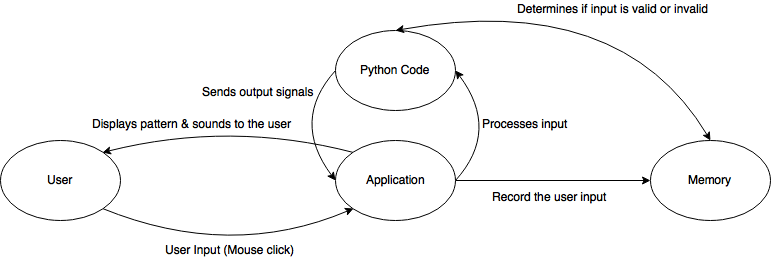
\includegraphics [width = \linewidth] {Context_Of_Work.png}
	\caption {Context of Work Diagram}
	\label {Figure: Context of Work}
\end {figure}
	

\subsubsection{Work Partitioning}
	
	\begin{table}[H]
		\centering
		\caption{List of Events}
		\label{tab:table2}
		\begin{tabular}{clll}
			\hline
			\# & Event & Input & Output\\
			\hline
			1. & DNA Says Creation & Developer code & Executable file\\
			2. & DNA Says Audio & Microphone & Audio output device\\
			3. & DNA Says GUI & Developer code & Monitor\\
			4. & Open the file & User input & New window\\
			5. & Select a mode & User input & Disks appear\\
			6. & Click a correct disk & User input & Light \& sound\\
			7. & Click an incorrect disk & User input & Sound\\
			8. & Repeat pattern successfully & User input & New pattern\\
			9. & Exit to main menu & User input & Main menu appears\\
			10. & Exit game & User input & Window termination\\
			\hline
		\end{tabular}
	\end{table}
	
\subsubsection{Individual Product Use Cases}

\begin{itemize}

\item Use Case \#1
\begin{itemize}
\item Name: Open the executable file.
\item Trigger: The user selects to open the file.
\item Precondition: The DNA Says icon must be available on the desktop.
\item Postcondition: The main menu will open.
\end{itemize}

\item Use Case \#2
\begin{itemize}
\item Name: Select a mode.
\item Trigger: The user selects to choose 1/3 modes.
\item Precondition: The user must be in the main menu.
\item Postcondition: The user will be able to view the 4 disks and begin the game.
\end{itemize}

\item Use Case \#3
\begin{itemize}
\item Name: Click a correct disk.
\item Trigger: The user selects a disk that was part of the pattern displayed. 
\item Precondition: The user must be in a mode and the computer has displayed the pattern.
\item Postcondition: The disk will light up and make a sound.
\end{itemize}

\item Use Case \#4
\begin{itemize}
\item Name: Click an incorrect disk.
\item Trigger: The user selects a disk that was not part of the pattern displayed.
\item Precondition: The user must be in a mode and the computer has displayed the pattern.
\item Postcondition: The disk will make a specific sound indicating an incorrect move and the correct disk will light up.
\end{itemize}

\item Use Case \#5
\begin{itemize}
\item Name: Successfully repeat the pattern.
\item Trigger: The user selects the series of disks that composed the pattern displayed.
\item Precondition: The user must be in a mode and the computer has displayed the pattern.
\item Postcondition: The next pattern will be displayed to the user.
\end{itemize}

\item Use Case \#6
\begin{itemize}
\item Name: Exit to the main menu.
\item Trigger: The user selects main menu icon.
\item Precondition: The user must be in a mode. 
\item Postcondition: The user will leave a mode and the main menu will open.
\end{itemize}

\item Use Case \#7
\begin{itemize}
\item Name: Exit game.
\item Trigger: The user selects the exit game icon
\item Precondition: The user must be in the main menu. 
\item Postcondition: The appllicaion will be terminated
\end{itemize}

\end{itemize}

\subsection{Functional Requirements}

\begin{itemize}

\item Requirement \#1
\begin{itemize}
\item Description: The user will be able to open the executable file.
\item Rationale: The user must be able to open the game.
\item Fit Criterion: A new window will open on the users computer screen.
\end{itemize}

\item Requirement \#2
\begin{itemize}
\item Description: The game interface will open in a new window.
\item Rationale: The game will be operated in a separate window. 
\item Fit Criterion: A new window will appear on the users computer screen
\end{itemize}

\item Requirement \#3
\begin{itemize}
\item Description: The game will have 3 separate modes - Kareem Says, JP Says, and Shady Says.
\item Rationale: The game is designed to have 3 distinct modes.
\item Fit Criterion: The 3 different modes will be displayed in the main menu of the game. 
\end{itemize}

\item Requirement \#4
\begin{itemize}
\item Description: The user will be able to select 1 of 3 modes to play.
\item Rationale: The user must be able to play 1 mode at a time. 
\item Fit Criterion: The user will be able to select 1 of the 3 modes displayed in the main menu of the game.
\end{itemize}

\item Requirement \#5
\begin{itemize}
\item Description: The main menu will display the 3 different modes. 
\item Rationale: The user must be able to view which mode they wish to select.
\item Fit Criterion: Three distinct icons will be displayed in the main menu.
\end{itemize}

\item Requirement \#6
\begin{itemize}
\item Description: Four different coloured disks will be shown to the user during each mode.
\item Rationale: The game is designed to have four distinct disks.
\item Fit Criterion: When a user selects a mode - the 4 disks will be displayed. 
\end{itemize}

\item Requirement \#7
\begin{itemize}
\item Description: Each disk will light up and produce a different sound when clicked.
\item Rationale: This gives the user the ability to detect the pattern that will be displayed.
\item Fit Criterion: When the user clicks a button - the disk will light up and produce a sound.
\end{itemize}

\item Requirement \#8
\begin{itemize}
\item Description: The user will be able to exit the game at any time and go back to the main menu. 
\item Rationale: The user must have a means of exiting an ongoing game and return to the main menu.
\item Fit Criterion: When the user clicks the main menu button, they will find their screen in the main menu window.
\end{itemize}

\item Requirement \#9
\begin{itemize}
\item Description: Every time a user passes a level, the score goes up by 1 point.
\item Rationale: A record of a users score must be kept. 
\item Fit Criterion: At level N, the score = N.
\end{itemize}

\item Requirement \#10
\begin{itemize}
\item Description: Every time a user fails a level, the score is reset to 0.
\item Rationale: When a user fails a level - the game must restart from level 1.
\item Fit Criterion: Whenever the user makes a mistake, the score icon will reset to 0.
\end{itemize}

\item Requirement \#11
\begin{itemize}
\item Description: There will be a score icon in the bottom right corner.
\item Rationale: The user must be able to view their score.
\item Fit Criterion: When the user selects a mode, the score icon will be set to 0.
\end{itemize}

\item Requirement \#12
\begin{itemize}
\item Description: At level N, a random pattern of N disks will light up and be displayed to the user.
\item Rationale: The levels difficulty will increase as the levels progress.
\item Fit Criterion: During level 1, one random disk will light up and sound.
\end{itemize}

\item Requirement \#13
\begin{itemize}
\item Description: The user cannot click the disks while the pattern is being displayed. 
\item Rationale: The pattern must be displayed to the user in full effect.
\item Fit Criterion: The program will not record clicks the user inputs during this time.
\end{itemize}

\item Requirement \#14
\begin{itemize}
\item Description: The user will be able to click the disks once the pattern has been displayed. 
\item Rationale: The user must repeat the pattern correctly to pass the level
\item Fit Criterion: The program will monitor the users input clicks to determine if the entry is correct or not.
\end{itemize}

\item Requirement \#15
\begin{itemize}
\item Description: A level is passed if the user repeats the pattern correctly.
\item Rationale: The user will be able to progress through the game. 
\item Fit Criterion: The score will be increased by 1 when the user is successful.
\end{itemize}

\item Requirement \#16
\begin{itemize}
\item Description: If the user fails, the game will restart - I.e. N = 1.
\item Rationale: The user must restart from the beginning of the game when a mistake is made.
\item Fit Criterion: Whenever a mistake is made, the user will be directed to level 1.
\end{itemize}

\end{itemize}


\section{Non-functional Requirements}
\subsection{Look and Feel Requirements}
\subsection{Usability and Humanity Requirements}
\subsection{Performance Requirements}
\subsection{Operational and Environmental Requirements}
\subsection{Maintainability and Support Requirements}
\subsection{Security Requirements}
\subsection{Cultural Requirements}
\subsection{Legal Requirements}
\subsection{Health and Safety Requirements}
This section is not in the original Volere template, but health and safety are
issues that should be considered for every engineering project.
\section{Project Issues}
\subsection{Open Issues}
\subsection{Off-the-Shelf Solutions}
\subsection{New Problems}
\subsection{Tasks}
\subsection{Migration to the New Product}
\subsection{Risks}
\subsection{Costs}
\subsection{User Documentation and Training}
\subsection{Waiting Room}
\subsection{Ideas for Solutions}
\bibliographystyle{plainnat}
\bibliography{SRS}
\newpage
\section{Appendix}
This section has been added to the Volere template.  This is where you can place
additional information.
\subsection{Symbolic Parameters}
The definition of the requirements will likely call for SYMBOLIC\_CONSTANTS.
Their values are defined in this section for easy maintenance.
\end{document}